\section{Durchführung}
\label{sec:Durchführung}

\begin{figure}
  \centering
  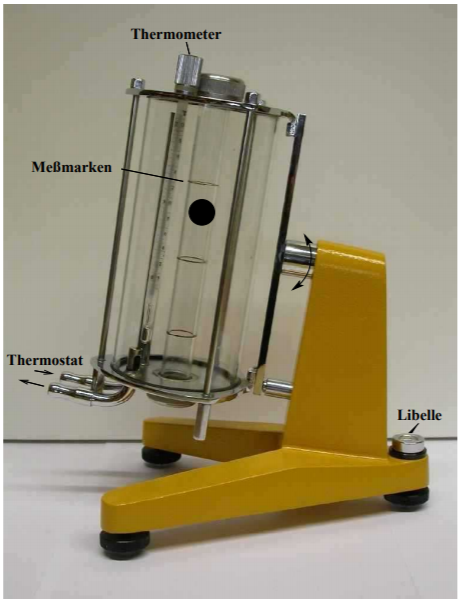
\includegraphics{content/viskosimeter.PNG}
  \caption{Kugelfall-Viskosimeter nach Höppler. \cite[2]{V207}}
  \label{fig:viskosimeter}
\end{figure}

Zunächst werden die Durchmesser und Massen der beiden Probekugeln gemessen. Die Kugeln selbst haben ungefähr dieselbe Größe wie das Rohr im Viskosimeter.

Das Viskosimeter wird gerade aufgestellt, dies wird mithilfe der eingebauten Libelle erreicht.

In \autoref{fig:viskosimeter} ist ein Kugelfall-Viskosimeter nach Höppler zu sehen. In das Glasrohr in der Mitte wird destilliertes Wasser gefüllt. Um dieses herum, befindet sich ein Behälter mir Wasser, das im Laufe des Experimentes erhitzt wird, um so indirekt auch die Temperatur von dem destilliertem Wasser zu erhöhen.
Während des gesamten Versuches ist darauf zu achten, dass sich keine Luftblasen im destillierten Wasser befinden, da sie zusätzlichen Auftrieb erzeugen würden und so die Messung verfälschen.

Es wird zunächst die kleinere Kugel in das Rohr gegeben. Anschließend wird das Rohr verschlossen und das System gedreht, sodass die Kugel im Wasser heruntersinkt.
Es wird angenommen, dass die Kugel ab der ersten Makierung eine konstante Geschwindigkeit erreicht hat und ab dieser wird die Zeit gemessen, die die Kugel benötigt, um die unterste Makierung zu erreichen. Die unterste und die oberste Makierung sind 100mm von einander entfernt.
Diese Messung wird insgesamt zehn mal wiederholt und anschließend wiederum zehn mal mit der größeren Kugel durchgeführt.

Die nächste Messreihe beschäftigt sich mit der Tempreaturabhängigkeit der Viskosität. Mithilfe eines Thermostates kann das Wasser im Viskosimeter erhitzt werden. Die jeweilige Temperatur wird mit einem Thermometer aufgenommen.
Die oben beschriebene Messung wird bei insgesamt zehn verschiedenen Temperaturen erneut durchgeführt. Dabei werden zu jeder Temperatur die Fallzeiten je zwei mal gemessen.
Während die Temperatur steigt, wird die Entlüftungsschraube am Viskosimeter gelockert, sodass der Druck im Inneren des Rohres nicht zu groß wird.
Diese Messreihe wird bis zu einer Temperatur von 70°C durchgeführt.
